\documentclass[twocolumn]{revtex4}
\usepackage{graphics,graphicx,epsfig,amsmath,multirow,gensymb,commath,textcomp,natbib,blindtext,mhchem,tabularx,array,makecell,threeparttable,amssymb}
\usepackage[a4paper, left=1.85cm, right=1.85cm, top=1.85cm, bottom=1.85cm]{geometry}   
\usepackage[normalem]{ulem}
\newcommand{\squeezeup}{\vspace{-2.5mm}}

\def\bibsection{\section*{\refname}} 
\renewcommand{\thesubsection}{\alph{subsection}}

\renewcommand\theadalign{bc}
\renewcommand\theadfont{\bfseries}
\renewcommand\theadgape{\Gape[4pt]}
\renewcommand\cellgape{\Gape[4pt]}

\begin{document}

\textheight=26.385cm
%Change textheight as the last resort...

\title{Observing Type Ia supernovae and fitting templated light curves}
 
\author{Jacky Cao, AstroLabs Michaelmas, Lab Partner: Duncan Middlemiss \\ Dates of experiment: 19/10/2017 to 08/12/2017, Date of report: 05/01/2018}

\begin{abstract}              
We have measured the magnitude of supernova explosions over an extended period of 34 days using $0.5$ m and $?.?$ m telescopes situated in Durham and La Palma. We have plotted several light curves and identified Type Ia, Type II, and ?? supernovae. Our fittings have had $\chi^2$ analysis has performed, and it has produced values of ?, ?, ?. We expect our biggest source of uncertainty arose due to the conditions and data analysis that we performed. Using a Type Ia supernova of brightness $00.00$ mag, we have managed to produce a value for Hubble's Constant, $H_0 = 74$ kms$^{-1}$ Mpc$^{-1}$. We attempted to calculate Einstein's coefficient, $\Lambda$, but this was unsuccessful due to redshift of something.
\end{abstract}

\maketitle

\vspace{-3ex}
\section{Introduction} 
\label{intro}
\vspace{-2ex}
In astronomy, one of the most violent and luminous events which can occur are supernova explosions. At the end of a massive star's lifetime, as a star runs out of nuclear fuel to burn, there is a possibility that the equilibrium configurations for a star will cease to exist. This leads to a final cataclysmic event, a supernova explosion. The luminosity of such, when at it's peak, can be as bright as a small galaxy \cite{longair}.

Observing these events and measuring their magnitude over a period of time allows us to plot light curves. The likes of which can then be used to visualise the evolution of a supernova. Using these plots we can draw the conclusion that there is order in the explosions. We find that if our sample of supernovae is large enough, we see that they can be grouped together into different types just by features from their light curves. The two general types of supernova are Type I and Type II, the difference between them being that Type I lacks the Balmer hydrogen features in it's spectra \cite{longair}, and that Type II events are very hydrogen-rich \cite{obs_phys_class_sn}.

\vspace{-3ex}
\subsection{Supernovae Classification}
\vspace{-2ex}

If we were to further study the light curve shapes and also the spectra of the supernovae from our sample, we would begin to recognise that there are further sub-classifications within Type I and Type II. In Table \ref{sn_classes} some of these subtypes are specified.

\begin{table}[h!]
\centering
\begin{tabular}{c@{\hskip 20pt}c} 
 \hline
 \textbf{Type} & \textbf{Characteristic} \\ 
 Ia		& Si II line present at $616.0$ nm in spectra \\
 Ia-91bg	& Absorption trough at $400-450$ nm in spectra \\
 		& \em Type Ib and Type Ic also exist \em \\
 IIP 		& Reaches a plateau in it's light curve  \\
 IIL		& Rapid linear decrease in light curve \\
 		& \em Type IIn and Type IIb also exist \em \\
 \hline
\end{tabular}
\caption{Some of the subclassifications of supernova and their respective characteristics which distinguish between them from each other \cite{longair, obs_phys_class_sn}.}
\label{sn_classes}
\end{table}

In the application to cosmology one of the most used types of supernovae are Type Ia, their light curve profiles are generally homogenous which allows them to be used as standard candles, thus providing a reliable distance indicator.  

We can see this homogeneity in Figure \ref{typeia-standard}. This plot was produced by superimposing and translating multiple sets of Type Ia data. The light curves in the B and V bands follow a general path in their evolution: they initially increase in brightness until they reach a peak magnitude, after this point the magnitude of the supernova decreases until no noticeable change can be detected by our telescopes. We note that whilst Type Ia's do peak at different magnitudes in when observed from in different bands, it is not as pronounced as is shown in Figure \ref{typeia-standard}.

\squeezeup
\begin{figure}[!h]
\begin{center}
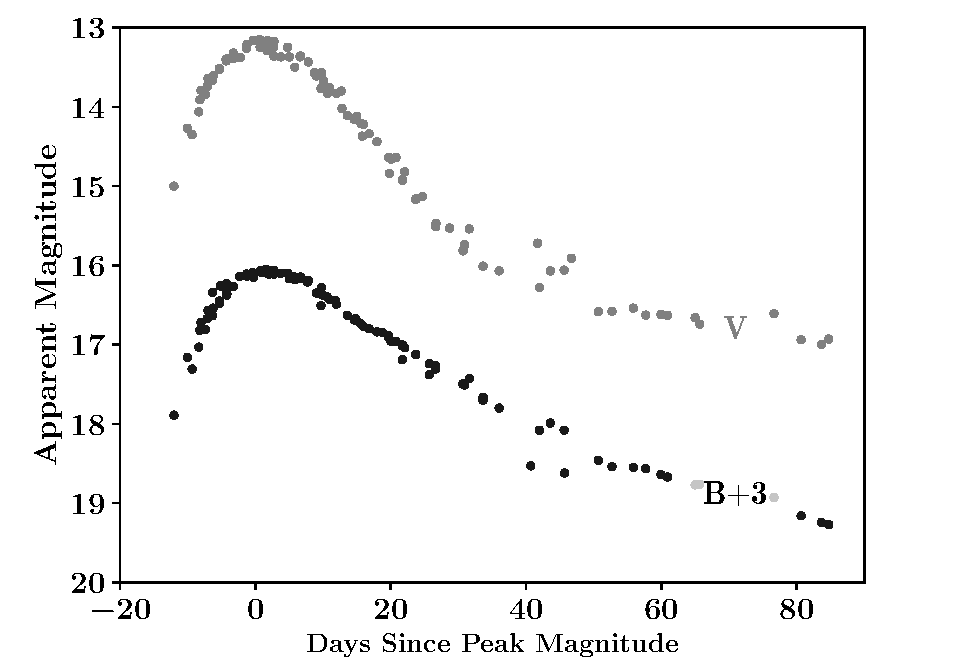
\includegraphics[width=9.25cm]{intro/typeia}
\caption[]{Plot showing the general forms of Type Ia supernovae in the B and V bands. Archival data was translated along the time axis and magnitude axis to produce the general forms of the light curves. The B band has been offset by a magnitude of $3$ to allow us to see both graphs clearly. The supernovae which were used to plot this graph are: \em{1994ae, 1994S, 1995bd, 1996bo, }\em  and \em{1998aq }\em \cite{jha, matheson}. }
\label{typeia-standard}
\end{center}
\end{figure}

In understanding the consistency of Type Ia light curves, we must attempt an exploration of the mechanisms of the explosion. This will involve developing an understanding of the system pre-supernova and also post-explosion.

The general consensus for Type Ia pre-supernova, as discussed by B. W. Carroll and D. A. Ostlie \cite{mod_ast}, is that a white dwarf within a binary system accretes matter from a donor star. However, this is also the initial system for dwarf novae and classical novae, which can grouped together as cataclysmic variables or novae. These too increase in brightness (classical novae by a factor of $\sim 10^6$ \cite{mod_ast}) which can lead to some confusion with supernovae, especially if you observe them optically without following up with any spectroscopic observations. 

It is understood that the difference which leads to cataclysmic variables and Type Ia supernovae is the process of accretion. This is dependent on the binary companion star, if the secondary star is on the main sequence then the white dwarf would just be steadily burning hydrogen or helium in it's surface layers, thus we would have a cataclysmic variable. To produce a supernova explosion we require a progenitor star to increase in mass towards the Chandrasekhar limit of $1.4$ $M_{\odot}$ \cite{posn, longair}. 

If the primary white dwarf was to accrete matter continually from it's binary companion until it itself was brought close to and past the critical mass, then a collapse to a neutron star must occur. However for a Type Ia supernova explosion this is not the case, before the collapse, the star is disrupted by large amounts of energy due to fusion reactions.

We can attribute this energy release to the fusion of carbon and oxygen within the core of the white dwarf. As material is continually accreted and compressed onto the surface, the star is heated and the temperature increases to $T \geq 10^9$ K \cite{longair}. When the thermonuclear energy is released, the white dwarf loses it's electron degeneracy pressure, and so becomes gravitationally unstable \cite{longair}. However, this energy that is produced disrupts the star and prevents the total collapse into a neutron star, this disruption leads to a supernova explosion \cite{posn}. 

In performing spectroscopic observations of Type Ia supernovae at maximum light we see that intermediate mass elements such as silicon, calcium, magnesium, sulphur, and oxygen are present which supports the picture of thermonuclear disruption \cite{longair, mod_ast}.

The process continues until the heaviest element that nuclear fusion can produce is made, iron. This is created from nickel capturing an electron through electron-capture (ec) into cobalt, and then the cobalt captures an electron and $\beta^{+}$ decays into iron \cite{mod_ast}. The process can be summarised in the following equation:
\begin{equation*}
\ce{^{56}Ni} \xrightarrow{\text{ec}} \ce{^{56}Co} \xrightarrow{\text{ec, $\beta^{+}$}} \ce{^{56}Fe}.
\end{equation*}

With these processes, they can be used to explain the form of the Type Ia light curves. The luminosity at peak maximum can be explained as the energy which has been deposited into the expanding envelope from the decay of the \ce{^{56}Ni} nuclei \cite{mod_ast}. We can highlight other features as seen in Figure \ref{typeia-standard}: the increase to peak magnitude is a fast process, it increases roughly half a magnitude a day; and the maximum of the light curve can be approximated as a Gaussian function \cite{mod_ast}. 

However, there are some peculiar types of Type Ia supernovae. For example, as featured in Table \ref{sn_classes}, Type Ia-91bg are a class of supernovae which have spectra which resembles those of Type Ia, however, they have an absorption band at $400-450$ nm. This arises due to a blend of Fe-group elements which is dominated by Ti II \cite{obs_phys_class_sn}. With their light curves they also lack the secondary maximum as found in normal Type Ia's within the I and R bands.

Observing objects and recognising that they are Type Ia supernovae thus requires not only spectroscopic observations but also observations in the optical. 

\vspace{-3ex}
\subsection{Supernova Discovery}
\vspace{-2ex}
In attempting to discover supernovae it is important that the search is not confined to a single region of the sky, whilst it may be possible to discover one of these events within that region, it would perhaps take a very long time until you could actually witness and collect data on it. What is thus required is a survey which spans the entire sky. 

A general method which can be employed to discover new supernovae is one which involves data comparison. If a survey takes an image of the entire night sky for every night, then to find new supernovae all that would be required is to subtract one night's data from the previous' and any objects which remain would be objects that could be new supernovae \cite{assasn-rev}. In reality it is not that simple, frames need to be cleaned of noise and they also require to be transformed in response to the point spread function. Plus, follow up observations would have to be made to verify if the object is supernovae or whether it is an anomalous object such as a cataclysmic variable. 

One such survey which employs this is the \em{All-Sky Automated Survey for Supernovae }\em (or ASAS-SN). Built up of five observations stations around the world, they produce a coverage of around $48,000$ square degrees of the night sky and they allow us to see up to a depth of $\sim 17$ mag \cite{asn_lc}, ASAS-SN is able to find many more supernovae and also supernovae which are close to the cores of galaxies, vastly increasing the discovery rate of bright supernova explosions and improving our understanding of where these events occur.

However, the majority of the supernovae are close enough to the detection limit that they need to be validated by other astronomers \cite{asn_lc}. This human review of transients has led to projects such as \textit{Supernova Hunters} \cite{cit-sci}, a citizen science program where volunteers are asked to classify objects which could be potential supernova candidates.  

These programs do not detract from the work that astronomers have to perform in the classification of supernovae, but it is equally important as it allows for the improvement of neural networks so that automatic surveys such as ASAS-SN can work more autonomously and efficiently \cite{cit-sci}.  

In all of this, we must keep in mind that telescopes are the key instruments in observing supernovae, or any astronomical object for that matter. To view objects which are 

\vspace{-3ex}
\subsection{Application to Cosmology} \label{appcosmo}
\vspace{-2ex}
Once we have our optical observations of Type Ia supernovae, we can then proceed to produce light curves and use them for cosmology. 

In discovering supernovae we can calculate the rates at which supernovae occur. Surveying different parts of the sky we can produce an estimate for the rate at which supernova explosions happen.

They expect to see $\sim 200$ Type Ia supernovae per year \cite{assasn-rev}, 

Using samples of nearby (redshift $z \lesssim0.1$) Type Ia supernovae, we can derive a value for Hubble's Constant, $H_0$, by plotting them on a a Hubble diagram \cite{exp_uni_sn}. It would also be possible to use Type Ia's to provide statistical constraints on cosmological models, for example with an $\Omega_M$, $\Omega_{\Lambda}$ Universe (where $\Omega_M$ is the mass density which includes ordinary and dark matter, and $\Omega_{\Lambda}$ is the effective mass density of dark energy) \cite{mod_ast, exp_uni_sn}. On top of that you, could measure the time-averaged equation of state of dark energy \cite{sn_consts}, $w$, a value which can be used to characterise the state of the universe. For an accelerating, dark energy dominated universe we would find that $w \approx -1$ \cite{longair}. [[paragraph to use as a basis for this section]]

When plotting their magnitudes against time passed we see that their light curves are generally homogeneous. These objects are the most luminous supernovae known, their absolute magnitudes in the B band are typically $M_B = -19.5 \pm 0.1$ \cite{posn}. Using light curve relationships and models we can determine precisely the magnitudes of very distant SNe, this has allowed astronomers to determine the redshift-distance relation for redshifts high redshift objects ($z>1$). Then, with these calculated values it is then possible to estimate the cosmological parameters $\Omega_0$ and $\Omega_\Lambda$. In doing so, it has been found that using Type Ia SNe has produced agreement with the literature value. so and so (cite paper) have done this and produced values of. 

asdasd \cite{abs_phil}
\begin{equation}
v = H_0 d, 
\end{equation}
with $v$ as the velocity of the receding object, $H_0$ as the value for Hubble's 
find a reference for this.

\vspace{-3ex}
\subsection{Project Aims}
\vspace{-2ex}
This paper outlines the study that was undertaken in an attempt to understand the evolution of the magnitudes of different supernovae over a time period [[?]]. From collected data it would be possible to produce light curves which we can use to identify the type of supernova that we were observing. In also understanding the uncertainties further analysis could be performed such as galaxy subtraction or [[think of something for here...]].

Section \ref{obsver} describes the methods used to collect and analyse the data, plus the uncertainties that arise during the experiment and how they were dealt with. Our final light curves, and the methods that were used to fit these models to the observations is summarised in Section \ref{analysis}. Section \ref{discussion} discusses the different blahj blah blah, and explores potential work that could be performed. With Section \ref{conclusions} provididng a summary and conlusion.

We also focussed on understanding the sources of uncertainties and attempted to reduce them within our analysis to produce magnitudes which would be more true to what they should be [[?]]. 

\vspace{-3ex}
\section{Observations} 
\label{obsver}
\vspace{-2ex}
\subsection{Data Collection}
\vspace{-2ex}

Observing supernova explosions requires instruments which are sensitive enough to receive the photons which have travelled for vast distances before being recorded. In performing such observations (?) our main equipment are telescopes - they come in a wide variety of configurations and each can produce different results.

In collecting the data for our supernova we used three different types of telescopes. Two of them based in Durham on the Department of Physic's Roof, and one in La Palma. 

As we were observing objects which were faint we required that we either have a large telescope to collect as much light as possible [reference], or have good seeing conditions which allowed us to collect as much light as possible over a large observation time.

In performing our observations, Far-East-16 and pt5m (give basic broad descriptions of these telescopes - tell how they are big and thus how much light they can collect?) was used. 

Talk about the CCDs, their specs, and what that implies. Any uncertainties work should be either stated here, or in the uncertainties section, or spoken about in both. 

Reliant on weather conditions being acceptable to observe in, define acceptable, discuss clouds, seeing, atmospheric turbulence, Lumiere, temperature, ...etc

in observations how has the moon affected us


\vspace{-3ex}
\subsection{Observations Made}
\vspace{-2ex}

Over a period of (?) days we took images of SNe, however this also depended on the conditions and whether it was worth observing if the seeing was bad e.g. obscured by bad weather.

In making observations there were various factors which required to be known.

In Appendix \ref{objectslog} is detailed all the objects that we chose to view over our experimental period, and in Appendix \ref{obslogs} is a more detailed description of the data that we took.

\vspace{-3ex}
\subsection{Data Analysis}
\vspace{-2ex}

[[WHAT TENSE AM I SUPPOSED TO USE? PAST OR PRESENT??]]

As we collected our supernova data over our experimental period we were then required to perform various photometry techniques to calculate the magnitudes of the explosions. It is important that this method was correct as we wanted accurate representations of the light curves. 

With our \em{raw}\em data we firstly needed to identify our supernova object, as these objects can blend in with the background of stars we had to look it up for the right ascension and declination reference. All of our supernova objects were discovered by other astronomers so they had an initial set of information we could use like, astronomical location on the celestial sphere, initial magnitude and the discovery date.

Once we had found our object we needed to find the magnitude of it. Using an astronomical analysis package such as GAIA [[reference and improve this]], we used various tools to perform this. We had to understand that we wanted to find the absolute magnitude of the supernova, this value being the 'actual magnitude', and not relative to other objects [[?]]. To perform this we had to choose at least two calibration stars which have known absolute magnitiudes.

To count the number of counts that we are receiving from our supernova and calibration objects we have to choose an apperture size to place over these objects. It is important thatthe radius that is chosen maximises the signal whilst reducing the amount of noise that we are receving as well, it is important that we have the cleanest signal possible.

To do this an object was selected which was close to the supernova and appeared to be similar in size, this was normally one of the calibration stars that we would be using. With our software package [[and for astronomy?]] we also had to choose a size for the 'sky aperture', this was so that the sky noise could be removed from the counts as well. In choosing this we had to account for the proximity of the supernova to its host galaxy's nucleus and also on how close the calibration stars are to other stars. We did not want to include unnecessary data that would produce an erroneous result. 

After a sky aperture had been chosen we would then try and find the best radius to use when doing our photometry. This radius would be constant for our calibration objects and for our supernova as well, and also for each day's data frames. This would ensure that we would be not 'cherrypicking' the signal that we are receving and that it would be an 'equal opportunity' for the signal to be detected to be the same each time [[??]]. 

This radius would be chosen by adjusting it from one to twenty in integer steps of one, noting down number of counts, the uncertainty on that value, and the sky noise counts. After these values had been collected we would plot the signal to noise against radius. In the plot, where the graph reaches a peak and decreases after this pooint would be our radius size as this would be the radius where we would achieve maximum signal to noise.

Then we can collect the values for the counts of the supernova and calibration objects, once we have this data we can use equation \ref{mag_counts} to find the absolute magnitude of the supernova. [[give a reference for the equation from a paper]]

\begin{equation}
    m = z - 2.5 \log_{10}{C},
\label{mag_counts}
\end{equation}

where $m$ is the absolute magnitude that we are trying to find, $z$ is the 'zero-point' of our frame [[is it how much it's offset by??]], and $C$ is the number of counts we receive from our object.

In using this equation we must have the correct zero-point, $z$, otherwise we would not be finding the absolute magnitude, instead the apparent magnitude relative to our calibration stars. So, rearranging the equation for $z$ we can calculate the zero-points for the calibration objects in the required observation bands. We have the counts for each object and we have their known magntidue which has been found by other astronomers. Then we can average the $z$-values togehter for their respective bands. 

With this $z$ value we can then use the form of the equation as given in equation \ref{mag_counts} and calculate the absolute magnitude of our supernovae.

Now with our magnitude values and the date that the data was taken on, we can plot a basic light curve. 

In fitting templates and models it can be manually done, or you could use a software package light \em{SNooPy }\em. All it requires is the data, redshift, and the right ascension and declination of the supernova object. It will fit Type Ia templates to the data and then return what it thinks is the best fitting.

Once we had collected our data we then proceeded to perform analysis

Data reduction, what was required, blah blah blah. What was used. Don't say dstack script, say a script was used which allowed us to stack images together. should i just blend uncertainties into here? 

fitting supernova templates using python programs, SNoopy - in depth analysis of snoopy should not be mentioned here, probably not

understanding type ia models of data and how from our data we cannot be sure.  
 cb
Photometry work 

\vspace{-3ex}
\subsection{Data Uncertainties}
\vspace{-2ex}

Throughout the experiment it was important that we kept in mind the uncertainties which may arise from different areas of the experiment. Quantifying these errors allows us to judge whether the data and fittings that we created were good or not. 

Uncertainties from the CCD and those type of astronomy data noise: mention here their effect, and how they were dealt with. 

\vspace{-3ex}
\subsection{Final Data}
\vspace{-2ex}

Below is the final data set for supernova 2017hhz, and 2017hle. 

\begin{table}[h!]
\centering
\begin{tabular}{c@{\hskip 20pt}c@{\hskip 20pt}c@{\hskip 20pt}c@{\hskip 20pt}c} 
 \hline
 \textbf{Date Observed} & \textbf{$\boldsymbol{m_B}$} & \textbf{$\boldsymbol{\Delta{m_B}}$} & \textbf{$\boldsymbol{m_V}$} & \textbf{$\boldsymbol{\Delta{m_V}}$} \\ [0.5ex] 
 20/10/17 & 16.8 & 0.1 & 17.1 & 0.1 \\
 22/10/17 & 16.9 & 0.1 & 16.8 & 0.1 \\
 23/10/17 & 16.8 & 0.2 & 16.9 & 0.1 \\
 26/10/17 & 17.0 & 0.2 & 17.0 & 0.1 \\
 29/10/17 & 17.2 & 0.1 & 17.0 & 0.1 \\
 30/10/17 & 17.3 & 0.1 & 17.1 & 0.1 \\
 05/11/17 & 17.7 & 0.2 & 17.3 & 0.2 \\
 11/11/17 & 18.2 & 0.4 & 17.5 & 0.2 \\
 16/11/17 & 18.6 & 0.2 & 17.8 & 0.1 \\
 17/11/17 & 18.8 & 0.2 & 18.2 & 0.4 \\
 \hline
\end{tabular}
\caption{The B and V band magnitudes and their uncertainties for SNe 2017hhz on the given dates. The former values were calculated using equation \ref{eqn1} and the latter using equation \ref{eqn2}.}
\label{2017hhz-table}
\end{table}

\begin{table}[h!]
\centering
\begin{tabular}{c@{\hskip 20pt}c@{\hskip 20pt}c@{\hskip 20pt}c@{\hskip 20pt}c} 
 \hline
 \textbf{Date Observed} & \textbf{$\boldsymbol{m_B}$} & \textbf{$\boldsymbol{\Delta{m_B}}$} & \textbf{$\boldsymbol{m_V}$} & \textbf{$\boldsymbol{\Delta{m_V}}$} \\ [0.5ex] 
 26/10/17 & 17.8 & 0.3 & 16.8 & 0.1 \\
 29/10/17 & 18.4 & 0.2 & 17.0 & 0.1 \\
 30/10/17 & 18.6 & 0.2 & 17.1 & 0.1 \\
 16/11/17 & 19.5 & 0.3 & 18.9 & 0.2 \\
 17/11/17 & 19.3 & 0.4 & 18.7 & 0.3 \\
 18/11/17 & 19.6 & 0.5 & 18.7 & 0.3 \\
 \hline
\end{tabular}
\caption{The B and V band magnitudes and their uncertainties for SNe 2017hle on the given dates. The former values were calculated using equation \ref{eqn1} and the latter using equation \ref{eqn2}.}
\label{2017hle-table}
\end{table}

asdfsdfsadfsdf

\begin{figure}[!h]
\begin{center}
\includegraphics[width=8.25cm]{images/collage_rectangle}
\caption[]{Images of the supernova 2017hhz, it's host galaxy, and the surrounding area. (a) Data was taken on the 20th October 2017. The calibration stars that were chosen have been labelled, 1 corresponds to star 512-002598, and 2 to 512-002599. These classifications were taken from the UCAC4 Catalog [[reference]]. The supernova 2017hhz has been shown with an arrow and label SNe. (b) Data from 23rd November 2017. (c) Data has been flat fielded for the 23rd November 2017. (d) An attempt has been made to remove the background galaxy for the data from 20th October 2017.}
\label{2017hhz_collage}
\end{center}
\end{figure}

\vspace{-3ex}
\section{Analysis}
\label{analysis}
\vspace{-2ex}
\subsection{Supernovae Models}
\vspace{-2ex}
In fitting the supernova templates to our data sets we used the software package SNooPy

Discuss how SNooPy fit's its models here? \cite{car_snoopy}

Usage of different models, if I can, find different models and fit them to our data and see how it would differ. What kind of techniques would be required to do so. 


\vspace{-3ex}
\subsection{Results}
\vspace{-2ex}

sdfsdfsa

\begin{figure}[!h]
\begin{center}
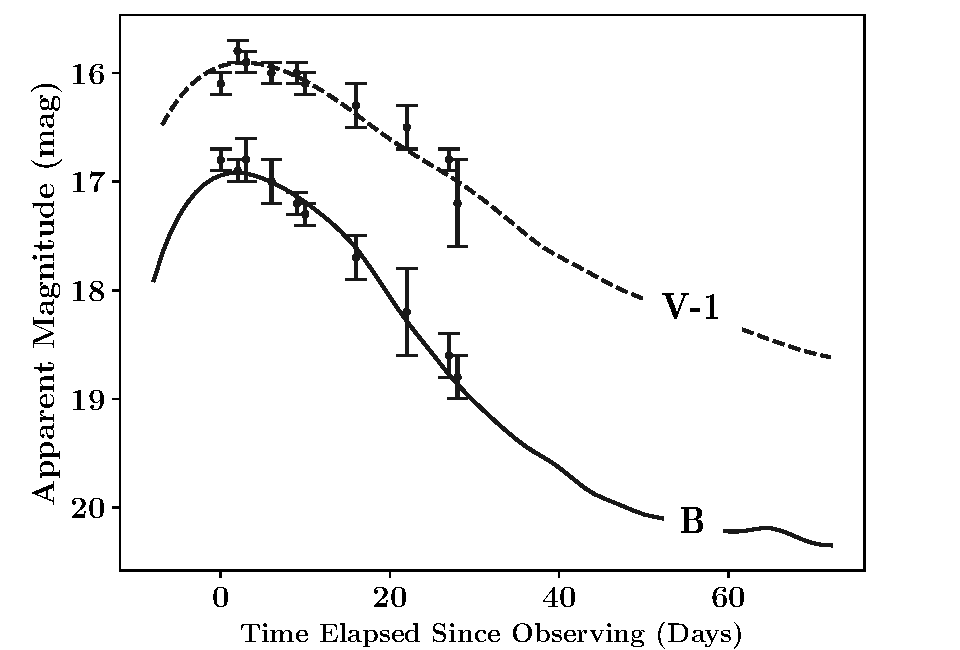
\includegraphics[width=9.25cm]{results/2017hhz}
\caption[]{The light curves for supernova 2017hhz. In the B band, the data has been plotted with the uncertainty in the magnitude plotted as well. The first observation, for day zero, was made on Friday 20th October 2017.}
\label{2017hhz-data}
\end{center}
\end{figure}

\begin{figure}[!h]
\begin{center}
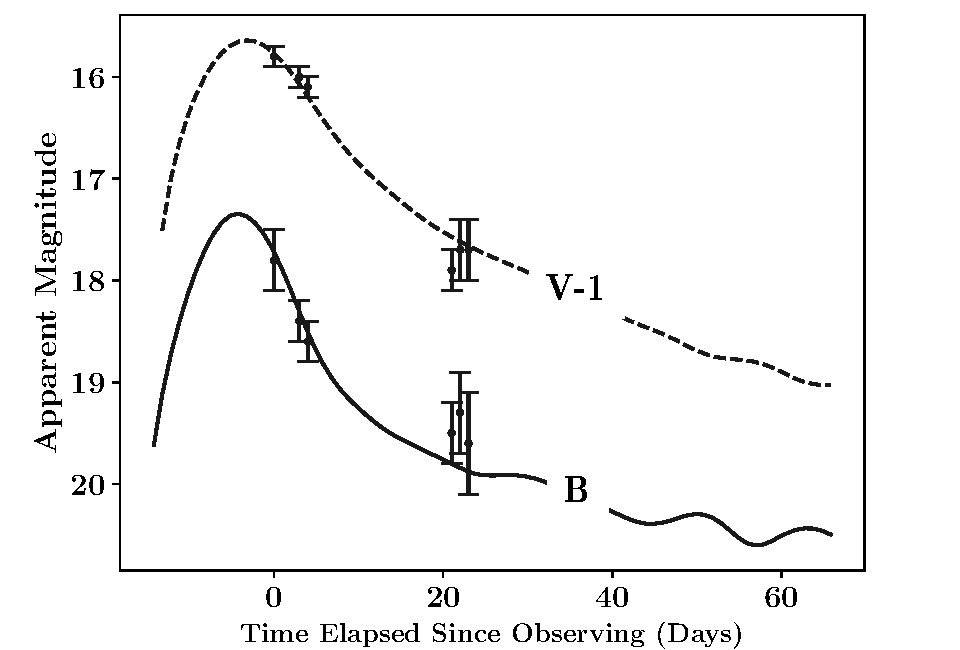
\includegraphics[width=9.25cm]{results/2017hle}
\caption[]{The light curves for supernova 2017hle. In the B band, the data has been plotted with the uncertainty in the magnitude plotted as well, }
\label{2017hle-data}
\end{center}
\end{figure}

\begin{table}[h!]
\centering
\begin{tabular}{c@{\hskip 20pt}c@{\hskip 20pt}c} 
 \hline
 \textbf{Supernova} & \textbf{$\boldsymbol{\chi^2}$} & \textbf{$\boldsymbol{\chi^2_{\nu}}$} \\ [0.5ex] 
 2017hhz & 1 & 1 \\
 2017hle & 2 & 2 \\
 \hline
\end{tabular}
\caption{$\chi^2$ and $\chi^2_{\nu}$ values that have been calculated for supernovae 2017hhz and 2017hle.}
\label{chi2-table}
\end{table}

\begin{figure}[!h]
\begin{center}
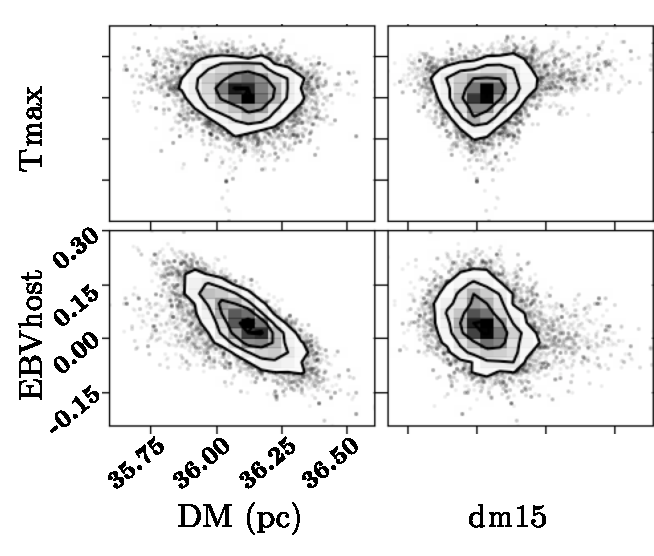
\includegraphics[width=7.5cm]{results/covariance/covariance}
\caption[]{Covariance between four variables, [[give them]], state which ones have been excluded and why we chose to view these one. These plots were produced using the fitMCMC function in SNooPy and they used the B and V band data for supernova 2017hhz.}
\label{2017hle-data}
\end{center}
\end{figure}

\vspace{-3ex}
\section{Discussion}
\label{discussion}
\vspace{-2ex}

\subsection{Using SNooPy to fit templates to supernovae}
SNooPy uses the Levenberg-Marquardt least-squares fitter to fit the model to the data [[cite]]. 

\subsection{Observing supernovae}
sdasd

\subsection{Supernovae in cosmology}

It is highly unlikely that we will see supernova remnants for the supernova that we have been studying, in the shape of the Crab Nebula. Much longer time periods would be required for this. 

In observing objects which are so faint we have the problem of trying to observe them. We need to balance the observing time to ensure that we do not oversaturate our frame with other stars. From the databases that we use, for this observation period the majority of our objects had been around the magnitudes of $\sim 18$ mag. But, we do not achieve this magnitude as there are various factors such as extinction affectinb data collection. 

We can calculate the limitiing magnitude that our telescopes could detect by analysing our frames

[neutrino studying]?



in using snoopy, how does it really fit the models to the data, what kind of parameters does it constrain. what is it's reliance on different parameters

try and produce some sort of covariance relation plot?

performing incorrect photometry and how that affects our results - not realising that we had to set a zero point, then having to find the zero point ourselves. 

confusion in observations, novae, cataclysmic variables 

there are other scripts which provide an automated way in finding the zero points from the data. what would this produce? why would this be beneficial to use this as opposed to our method?

justification of using the uncertainty equation, functional approach, why not use the uncertainty that was provided by the software? mention how it's one of the photon statistics things.

dstack, taking the median not mean , and why this is better - if I haven't discussed this already

what science have we addressed? well, we have limitations on the telescopes in terms of how 'deep' we can see:  the limiting magnitude, how that was calculated - longer exposure times...etc

has it been possible to plot a light curve with reasonable uncertainties? how best could this experiment be changed? 

big picture: justification of the uncertainties 

using the jackknife method to discover the range of uncertainties after we had used snoopy to fit a model, the whole different parameters relating to each other

statisitcal, experimental - different uncertainties

extinction and galaxy extinction taking them into calculations

hubble flow????

how using different fitting models to check the quality of the data, right now we haven't really explored the quality of our data. 

\subsection{Improvements and extensions}
How could we improve upon our experiment, what else could we work on for extension projects.

\vspace{-5ex}
\section{Conclusions}
\label{conclusions}
\vspace{-2ex}

sdfsdfasdas

\vspace{-5ex}
\section*{Acknowledgements}
\vspace{-2ex}
We thank J. Lucey, M. Swinbank, and U. Dudzeviciute for their continual support and help which was provided over our entire experimental period. We also thank the staff at the Department of Physics at Durham University for the continual upkeep of the telescopes on the department's roof, and we thank R. Wilson for the maintenance of the robotic telescope at La Palma.

This research has made use of the CfA Supernova Archive, which is funded in part by the National Science Foundation through grant AST 0907903.

\bibliographystyle{abbrv}
\bibliography{supernovae}

\clearpage
\onecolumngrid
\vspace{-3ex}
\section*{Appendix A - Objects Log} \label{objectslog}
\vspace{-2ex}
A list of the objects that were chosen to be observed, and then the subsequent notes on them. Not all objects were chosen to be observed for an extended period, the ones noted were observed for a couple of nights to ensure suitability. The subsequent observation logs can be found in Appendix B.

{\renewcommand{\arraystretch}{1.2}%
\begin{table}[h!]
\centering    
\begin{tabularx}{\textwidth}{c c c c @{\hskip 5pt} c c X}
    \hline
    \textbf{Object} & \textbf{RA} & \textbf{Dec} & \textbf{Magnitude} &\textbf{First Discovered} &\textbf{Type} & \textbf{Notes} \\ 
    *ASASSN-17mz & 23:56:21.82 & +32:27:24.08 & 14.6 & 2017/09/30.500 & Ia & {Too close to galactic nucleus, cannot see}  \\
    *AT2017hld & 22:18:22.849 & +34:45:08.46 & 16.1 & 2017/10/17.339 & CV & {Cataclysmic Variable, stopped observing}  \\
    *2017hky & 11:23:30.514 & +63:21:59.43 & 16.2 & 2017/10/16.640 & II & {Not viewable from Durham or La Palma}  \\
    2017hhz & 01:44:16.75 & +12:15:18.00 & 16.83 & 2017/10/16.140 & Ia & {A measured redshift, $z=0.0392$}  \\
    AT2017gvb & 08:04:42.34 & +61:31:41.50 & 17.33 & 2017/09/26.59 & unk & {-}  \\
    *ASASSN-17nb & 07:27:37.32 & +35:36:28.30 & 17.31 & 2017/09/25.59 & II & {Object is dwarfed by brightness of the galaxy}  \\
    2017hle & 01:07:36.060 & +32:24:30.00 & 18.0 & 2017/10/18.684 & Ia-91bg & {-}  \\
    2017hou & 04:09:02.140 & -01:09:36.40 & 17.9 & 2017/10/24.370 &Ia & {Viewable from La Palma}  \\
    *AT2017hmw & 01:07:16.570 & +31:25:28.88 & 17.2 & 2017/10/19.415 & CV & {Cataclysmic Variable}  \\
    2017hpa & 04:39:50.750 & +07:03:54.90 & 17.9 & 2017/10/15.346 & Ia & {Viewable from La Palma}  \\
    *AT2017hnm & 01:42:03.24 & +42:31:08.50 & 16.69 & 2017/10/23.44 & unk & {Another star in the image dwarfs the SN in brightness}  \\
    AT2017hpm & 08:04:15.100 & -00:03:58.03 & 16.4 & 2017/10/26.290 & unk & {-}  \\
    *AT2017hqa & 01:08:59.160 & +32:38:04.10 & 17.3 & 2017/10/26.740 & unk & {Unobservable, too close to galactic centre}  \\
    2017hqc & 23:23:08.210 & +10:38:54.63 & 18.0 & 2017/10/27.490 & Ia & {-}  \\
    *AT2017hrr & 11:29:06.490 & -08:59:18.56 & 15.4 & 2017/10/30.607 & unk & {Cannot view from Durham or La Palma}  \\
    *AT2017hhq & 00:42:50.230 & +41:15:27.10 & 17.7 & 2017/10/30.599 & NV & {A nova close to M31}  \\
    AT2017htb & 22:09:38.520 & +17:39:39.56 & 15.7 & 2017/11/02.190 & unk & {-}  \\
    AT2017hzw & 02:05:18.337 & +53:12:13.16 & 17.3 & 2017/11/13.410 & Ia-CSM & {-}  \\
    2017igf & 11:42:49.850 & +77:22:12.94 & 15.4 & 2017/11/18.590 & Ia & {-}  \\
    \hline      
\end{tabularx}
\caption{Objects that we chose to observe and notes on them. RA is the Right Ascension, given in units of hours : arcminutes : arcseconds. Dec is the Declination, degrees : minutes : seconds. The stated magnitude is the initial magnitude that the object was discovered in the V band. Objects marked with an asterisk $*$ were objects which we chose to stop observing, the reason provided in the notes.}
\label{objects}
\end{table}


\clearpage

\onecolumngrid
\vspace{-3ex}
\section*{Appendix B - Observation Logs} \label{obslogs}
\vspace{-2ex}
Given below are all the observations which were made during our observation periods. The exposures column is of the following format: ($x: y, z$ s), where $x$ is the band in which the images were taken in, $y$ the number of exposures taken, and $z$ the exposure time which was used, in units of seconds.
{\renewcommand{\arraystretch}{1.2}%
\begin{table}[h!]
\centering    
\begin{tabularx}{\textwidth}{c@{\hskip 5pt} c c@{\hskip 5pt} c@{\hskip 5pt} c@{\hskip 5pt} X}
    \hline
    \textbf{Date} & \textbf{Object} & \textbf{Time} & \textbf{Exposures} & \textbf{  Conditions  } & \textbf{Notes} \\ 
    20/10/17 & 2017hhz & 22:25:34 to 22:58:50 & \makecell{B: 5, 120s \\ V: 5, 120s} & {Clear} & {pt5m: -}  \\
    	& ASASSN-17nb &  02:56:08 to 03:23:36 & \makecell{B: 5, 60s \\ V: 5, 60s} & {Cloudy} & {pt5m: Data was unusable due to noise from cloud.} \\      
	
    21/10/17 & - & - & - & Cloudy & {\em No observations: weather not sufficient in Durham or La Palma for observations. \em} \\
    
    22/10/17 & AT2017hmw &  21:52:20 to 22:31:49 & \makecell{B: 5, 120s \\ V: 5, 120s} & {Clear} & {pt5m: -} \\  
    & 2017hhz & 22:40:20 to 23:19:50 & \makecell{B: 4, 60s \\ V: 12, 60s} & {Clear} & {pt5m: -}  \\
    & ASASSN-17nb &  02:42:45 to 03:10:46 & \makecell{B: 5, 120s \\ V: 5, 60s} & {Clear} & {pt5m: -} \\  
    & AT2017gvb & 03:12:31 to 03:58:58 & \makecell{B: 5, 180s \\ V: 5, 120s} & {Clear} & {pt5m: -} \\    
    
    23/10/17 & 2017hhz & 22:53:12 to 23:32:42 & \makecell{B: 5, 120s \\ V: 5, 120s} & {Cloudy} & {pt5m: Data produced has FWHM ranging from $1.6$ to $9.9$.} \\  
    
    24/10/17 & 2017hhz & 22:44:01 to 23:23:30 & \makecell{B: 5, 120s \\ V: 5, 120s} & {Cloudy} & {pt5m: Data is noisy, potentially another object transited across the frame while observing.} \\  
    
    25/10/17 & - & - & - & {Cloudy} & {\em No observations: too cloudy for observations in Durham, and items in pt5m queue were pushed out in favour of other objects. \em} \\
    
    26/10/17 & 2017hle & 20:54:44 to 21:09:03 & \makecell{B: 4, 60s \\ V: 4, 60s} & {Clear} & {FE16: - }  \\
    & 2017hhz &  21:18:00 to 21:25:31 & \makecell{B: 4, 60s \\ V: 4, 60s} & {Clear} & {FE16: -} \\ 
    & AT2017hmw &  21:29:15 to 21:39:36 & \makecell{B: 4, 60s \\ V: 4, 60s} & {Cloudy} & {FE16: -} \\
    & Messier-7 &  21:50:23 to 21:54:47 & {C: 1, 60s} & {Slightly Cloudy} & {FE16: Test object for SN discovery.} \\
    & Messier-10 &  21:55:47 to 22:00:13 & {C: 1, 60s} & {Cloudy} & {FE16: Test object for SN discovery.} \\
    & AT2017hnm &  23:27:22 to 23:41:55 & \makecell{B: 5, 120s \\ V: 3, 120s} & {Clear} & {pt5m: -} \\ 
    & AT2017gvb &  - & - & {-} & {pt5m: Object pushed out of the queue in favour of others.} \\

    27/10/17 & AT2017hqa & 18:48:12 to 18:52:59 & \makecell{B: 4, 60s} & {Cloudy} & {FE16: Object too close to galactic nucleus. }  \\
    & AT2017hnm &  18:56:34 to 19:00:23 & \makecell{C: 1, 60s} & {Slightly Cloudy} & {FE16: Object too dim, cloud cover reduced light we were receiving.} \\
    & Abell 426 &  19:04:23 to 19:15:41 & \makecell{C: 1, 60s \\ B: 9, 60s \\ V: 9, 60s} & {Clear} & {E14: Object to observe to discover new SN.} \\
    & 2017hhz &  20:11:35 to 20:22:43 & \makecell{B: 4, 60s \\ V: 4, 60s} & {Cloudy and Windy} & {E14: Seeing is bad due to the weather.} \\
    & 2017hle &  20:26:18 to 20:37:35 & \makecell{B: 4, 90s \\ V: 4, 90s} & {Slightly Cloudy} & {E14: Seeing is bad in these images as well.} \\
    & 2017hou &  23:48:09 to 23:50:14 & \makecell{B: 2, 120s} & {-} & {pt5m: Only two frames taken, not sufficient data.} \\
    \hline      
\end{tabularx}
\label{obs_logs1}
\end{table}

{\renewcommand{\arraystretch}{1.2}%
\begin{table}[h!]
\centering    
\begin{tabularx}{\textwidth}{c@{\hskip 5pt} c c@{\hskip 5pt} c@{\hskip 5pt} c@{\hskip 5pt} X}
    \hline
    \textbf{Date} & \textbf{Object} & \textbf{Time} & \textbf{Exposures} & \textbf{  Conditions  } & \textbf{Notes} \\ 
    27/10/17 & AT2017gvb &  02:16:01 to 03:03:05 & \makecell{B: 5, 120s \\ V: 5, 120s} & {Clear/Cloudy} & {pt5m: Some images are more noisy due to clouds.} \\
    
    28/10/17 & AT2017hnm &  21:41:55 to 22:21:25 & \makecell{B: 5, 120s \\ V: 5, 120s} & {Clear} & {pt5m: -} \\
    & 2017hhz &  21:28:50 to 21:30:50 & \makecell{B: 1, 120s} & {Clear} & {pt5m: -} \\
    
    29/10/17 & 2017hle &  21:22:39 to 21:41:21 & \makecell{B: 10, 120s \\ V: 1, 120s} & {Clear} & {pt5m: Mistake on our part to take so many images in B band, and only one in V band.} \\
    & AT2017hnm &  21:55:34 to 22:35:04 & \makecell{B: 5, 120s \\ V: 5, 120s} & {Slightly Cloudy} & {pt5m: -} \\
    & 2017hhz &  23:16:48 to 23:56:18 & \makecell{B: 5, 120s \\ V: 5, 120s} & {Clear} & {pt5m: -} \\
    & 2017hou &  00:33:33 to 01:13:02 & \makecell{B: 5, 120s \\ V: 5, 120s} & {Clear} & {pt5m: -} \\
    & 2017hqc &  01:16:20 to 01:41:20 & \makecell{B: 4, 120s \\ V: 4, 120s} & {Clear} & {pt5m: -} \\
    & AT2017gvb &  02:18:51 to 02:55:47 & \makecell{V: 13, 180s} & {Clear} & {pt5m: Long exposure and large number of exposures chosen as a test to see the quality of stacking them.} \\
    
    30/10/17 & 2017hle &  21:18:56 to 21:58:25 & \makecell{B: 10, 120s \\ V: 10, 120s} & {Clear} & {pt5m: -} \\
    & 2017hhz &  22:06:34 to 22:46:04 & \makecell{B: 5, 120s \\ V: 5, 120s} & {Clear} & {pt5m: -} \\
    & AT2017gvb &  02:04:22 to 03:02:50 & \makecell{V: 20, 180s} & {Clear} & {pt5m: An human error, we re-selected this object from the previous night instead of the one with the correct number of required frames for each band.} \\
    
    31/10/17 & - & - & - & {Cloudy} & {\em No observations: too cloudy for observations in Durham and La Palma. \em} \\
    
    01/11/17 & 2017hle & 23:56:53 to 00:15:35 & \makecell{B: 5, 120s \\ V: 5, 120s} & Clear & {pt5m: -} \\
    & AT2017hnm & 00:18:23 to 00:57:55 & \makecell{B: 5, 120s \\ V: 5, 120s} & Clear & {pt5m: -} \\
    & 2017hhz & 01:00:47 to 01:40:17 & \makecell{B: 5, 120s \\ V: 5, 120s} & Clear & {pt5m: -} \\
    & 2017hou & 01:43:38 to 02:23:08 & \makecell{B: 5, 120s \\ V: 5, 120s} & Clear & {pt5m: -} \\
    
    02/11/17 & - & - & - & {Cloudy} & {\em No observations: too cloudy for observations in Durham and La Palma. \em} \\
    
    03/11/17 & - & - & - & {Cloudy} & {\em No observations: too cloudy for observations in Durham and La Palma. \em} \\
    
    04/11/17 & - & - & - & {Cloudy} & {\em No observations: too cloudy for observations in Durham and La Palma. \em} \\
    
   05/11/17 & ASASSN-17mz & 17:53:45 to 18:09:34 & \makecell{B: 8, 60s \\ V: 8, 60s} & {Clear} & {FE16: -} \\
   & 2017hhz & 18:50:39 to 19:24:43 & \makecell{B: 8, 120s \\ V: 8, 60s} & {Clear} & {FE16: -} \\
   & AT2017htb & 19:38:14 to 20:02:16 & \makecell{B: 8, 60s \\ V: 8, 60s} & {Slightly Cloudy} & {W14: -} \\
   & 2017hle & 20:05:49 to 20:08:28 & \makecell{V: 2, 60s} & {Cloudy} & {W14: Stopped taking exposures after the weather worsened.} \\
   & 2017hqc & 20:14:16 to 20:18:25 & \makecell{V: 3, 60s} & {Cloudy} & {W14: Cleared up for a brief moment and then re-clouded over.} \\
   & AT2017hhq & 20:33:58 to 20:42:26 & \makecell{B: 4, 60s \\ V: 4, 60s} & {Clear} & {W14: -} \\
       \hline      
\end{tabularx}
\label{obs_logs2}
\end{table}

{\renewcommand{\arraystretch}{1.2}%
\begin{table}[h!]
\centering    
\begin{tabularx}{\textwidth}{c@{\hskip 5pt} c c@{\hskip 5pt} c@{\hskip 5pt} c@{\hskip 5pt} X}
    \hline
    \textbf{Date} & \textbf{Object} & \textbf{Time} & \textbf{Exposures} & \textbf{  Conditions  } & \textbf{Notes} \\ 
    05/11/17 & AT2017hhq & 19:38:14 to 20:02:16 & \makecell{B: 3, 30s \\ V: 3, 30s \\ R: 3, 30s} & {Cloudy} & {E14: Images taken so that we can produce a colour image. } \\
    
    06/11/17 & - & - & - & {Cloudy, and Rain} & {\em No observations: too cloudy for observations in Durham, and torrential rain in La Palma. \em} \\
    
    07/11/17 & - & - & - & {Cloudy and Rain} & {\em No observations: too cloudy for observations in Durham, and torrential rain in La Palma. \em} \\
    
    08/11/17 & - & - & - & {Cloudy and Rain} & {\em No observations: too cloudy for observations in Durham, and torrential rain in La Palma. \em} \\
    
    09/11/17 & - & - & - & {Cloudy} & {\em No observations: too cloudy for observations in Durham, La Palma was not functioning. \em} \\
    
    10/11/17 & 2017hhz & 19:15:32 to 19:31:57 & \makecell{B: 4, 90s \\ V: 2, 90s} & {Cloudy} & {FE16: -} \\
    & 2017hqc & 19:37:27 to 19:49:15 & \makecell{B: 4, 90s \\ V: 2, 90s} & {Cloudy} & {FE16: -} \\
    
    11/11/17 & AT2017htb & 19:08:41 to 19:26:15 & \makecell{B: 5, 60s \\ V: 8, 60s} & {Clear} & {FE16: -} \\
    & 2017hhz & 19:34:43 to 19:43:48 & \makecell{B: 5, 60s \\ V: 4, 60s} & {Clear} & {FE16: -} \\
    & 2017hle & 19:45:56 to 19:53:46 & \makecell{B: 4, 60s \\ V: 4, 60s} & {Clear} & {FE16: -} \\
    & 2017hqc & 19:55:31 to 20:02:59 & \makecell{B: 4, 60s \\ V: 4, 60s} & {Clear} & {FE16: -} \\
    & Abell 426 & 20:04:54 to 20:08:03 & \makecell{B: 4, 60s} & {Clear} & {FE16: -} \\
    & 2017hhz & 20:09:53 to 20:34:55 & \makecell{B: 15, 60s \\ V: 7, 60s} & {Clear} & {FE16: It was made clear that having more frames would improve the quality of the final stacked frame. So more frames for this supernova were made.} \\
    
    12/11/17 & 2017hhz & 20:35:15 to 20:53:08 & \makecell{V: 17, 60s} & {Clear} & {FE16: As the night progressed, conditions became more cloudy so we were unable to take in the B band.} \\
    & 2017hle & 21:03:54 to 21:22:36 & \makecell{B: 5: 120s \\ V: 5, 120s} & {Clear} & {pt5m: We decided to input our remaining targets into the telescope in La Palma for observation.} \\
    & 2017hqc & 21:26:00 to 21:57:13 & \makecell{B: 4: 120s \\ V: 4, 120s} & {Clear} & {pt5m: -} \\
    
    15/11/17 & 2017hhz & 21:01:09 to 21:40:40 & \makecell{B: 5, 120s \\ V: 5, 120s} & {Clear} & {pt5m: -} \\
    & 2017hou & 00:16:29 to 00:56:01 & \makecell{B: 4: 120s \\ V: 4, 120s} & {Clear} & {pt5m: -} \\
    & AT2017gvb & 01:33:35 to 02:32:04 & \makecell{V: 20, 180s} & {Clear} & {pt5m: We made a mistake with our entry into the telescope queue- we selected too high of an exposure number.} \\
    
    16/11/17 & 2017hhz & 19:19:46 to 20:11:30 & \makecell{B: 8, 180s \\ V: 8, 180s} & {Clear} & {FE16: -} \\
    & 2017hle & 20:20:05 to 20:48:31 & \makecell{B: 8, 90s \\ V: 8, 90s} & {Clear} & {FE16: -} \\
    & Abell 426 & 21:01:35 to 21:17:03 & \makecell{B: 18, 30s} & {Clear} & {FE16: -} \\
    
    17/11/17 & 2017hhz & 18:52:28 to 19:49:50 & \makecell{B: 8, 90s \\ V: 8, 90s} & {Clear} & {FE16: -} \\
    & 2017hle & 19:52:09 to 20:15:48 & \makecell{B: 8, 90s \\ V: 8, 90s} & {Clear} & {FE16: -} \\
    & AT2017htb & 20:18:47 to 20:29:42 & \makecell{B: 4, 90s \\ V: 4, 90s} & {Clear} & {FE16: -} \\
    
       \hline      
\end{tabularx}
\label{obs_logs3}
\end{table}

{\renewcommand{\arraystretch}{1.2}%
\begin{table}[h!]
\centering    
\begin{tabularx}{\textwidth}{c@{\hskip 5pt} c c@{\hskip 5pt} c@{\hskip 5pt} c@{\hskip 5pt} X}
    \hline
    \textbf{Date} & \textbf{Object} & \textbf{Time} & \textbf{Exposures} & \textbf{  Conditions  } & \textbf{Notes} \\ 
    17/11/17& AT2017hzw & 20:40:43 to 21:00:19 & \makecell{B: 16, 60s} & {Cloudy} & {FE16: Stopped observations as it had become cloudy.} \\
    
    18/11/17 & 2017hle & 18:13:52 to 19:01:03 & \makecell{B: 15, 60s \\ V: 24, 60s} & {Clear} & {FE16: -} \\
    & 2017hhz & 19:03:47 to 19:45:56 & \makecell{B: 16, 60s \\ V: 24, 60s} & {Clear} & {FE16: -} \\
    
    23/11/17 & 2017hhz & 19:38:31 to 20:34:04 & \makecell{B: 16, 60s \\ V: 24, 60s} & {Clear} & {FE16: -} \\
    & 2017hhz & 20:36:52 to 21:00:00 & \makecell{V: 15, 90s} & {Clear} & {FE16: Clouded over at the end of our observations for V band.} \\
       \hline      
\end{tabularx}
\caption{Observation logs for the entire observation period for our experiment.}
\label{obs_logs4}
\end{table}


\clearpage

\twocolumngrid
\vspace{-3ex}
\section*{Appendix C - Set of Sample Data}
\vspace{-2ex}

asdasda

\clearpage

\twocolumngrid
\vspace{-3ex}
\section*{Appendix D - Uncertainties}
\vspace{-2ex}

\end{document}
